\documentclass[12pt]{beamer}
\usepackage{beamerthemeHannover, graphicx, clrscode, amsmath, amssymb, multicol}
\usepackage{textcomp} \usepackage{verbatim}
\usepackage{listings}
\setbeamercolor{sidebar}{use=structure,bg=red!60!yellow}
\lstset{language=SQL}

\title{LearnFWD: Testing CASH Music}
\author[@dukeleto]{Jonathan "Duke" Leto}
\date{}

\begin{document}

\frame{
    \titlepage
    \begin{center}
    
\includegraphics[scale=0.5]{webfwd.jpg}
    \end{center}
}

\frame{
    \frametitle{What does CASH Music use to test stuff?}
    \begin{itemize}
        \item PHP SimpleTest - http://simpletest.org
        \item Test::WWW::Mechanize - http://cpan.org
        \item Test::Most - http://cpan.org
        \item Test::JSON - http://cpan.org
        \item Jitterbug - http://jitterbug.pl
    \end{itemize}
}

\frame{
    \frametitle{What is Continuous Integration (CI) ?}

    \begin{itemize}
    \item Continually and automatically testing code, usually with relevant notifications.
    \item http://dev.cashmusic.org:3000
    \end{itemize}
}

\frame{
    \frametitle{Why is CI Useful?}
    \begin{itemize}
        \item Know the exact commit that broke something
        \item Automate testing many different combinations of different versions
            of libraries, languages, OS's, browsers, etc...
        \item Quickly identifies tests that only pass on the authors machine
            due to implicit assumptions
    \end{itemize}
}

\frame{
    \frametitle{What problems does Jitterbug solve?}
    \begin{itemize}
        \item People forgetting to run the test suite
        \item People forgetting to notify others when they see breakage
        \item Not having a visual interface to which commits passed
            and which failed a test suite
    \end{itemize}
}

\frame{
    \frametitle{Current Jitterbug Features}
    \begin{itemize}
        \item Extremely Memory Efficient
        \item Integrates seamlessy with Github post-receive hooks
        \item Can autodetect test suites in many languages
        \item Highly customizable YAML configuration file
        \item Email+RSS notifiers
        \item Supports custom build/test scripts
        \item Pretty web interface
    \end{itemize}
}

\frame{
    \frametitle{What does Jitterbug look like? }

    \begin{center}
        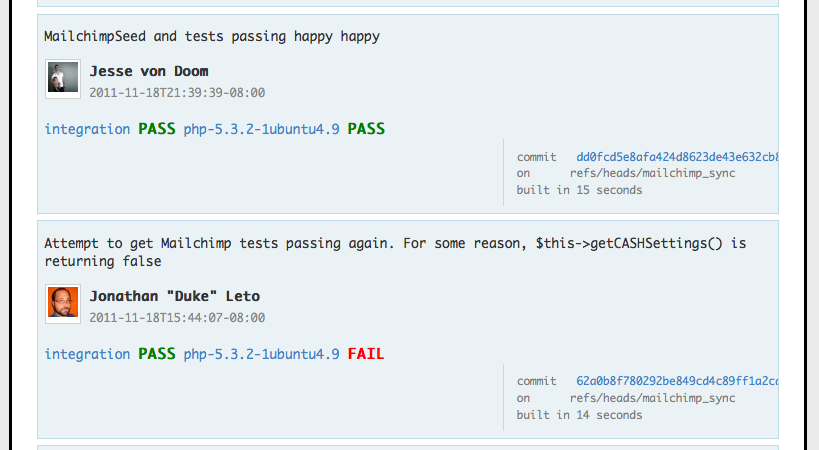
\includegraphics[scale=0.3]{cm_jitterbug2}
    \end{center}
}

\frame{
    \frametitle{What do our PHP tests look like?}
    \begin{center}
        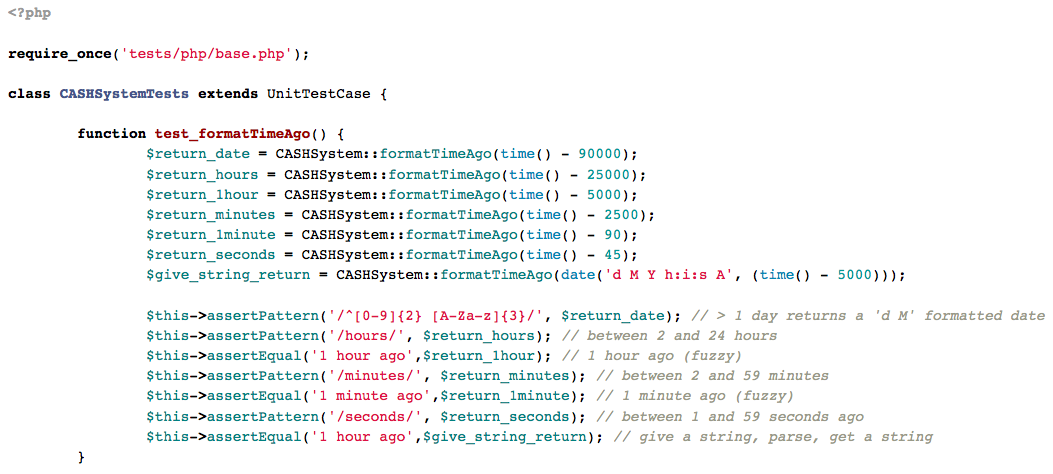
\includegraphics[scale=0.3]{cm_system_tests}
    \end{center}
}

\frame{
    \frametitle{What do our Perl tests look like?}
    \begin{center}
        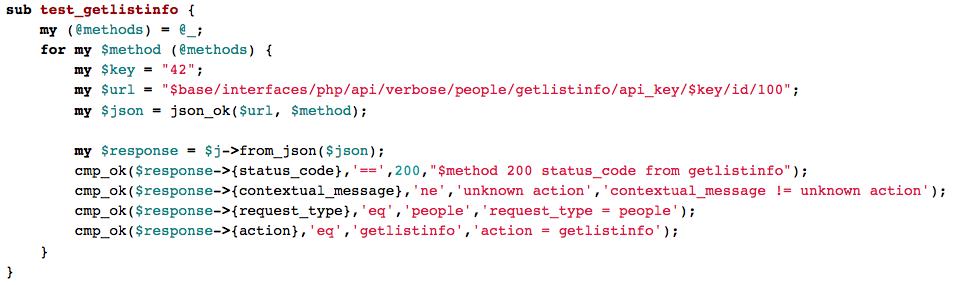
\includegraphics[scale=0.30]{cm_perl_test}
    \end{center}
}

\frame{
    \frametitle{What does passing test output look like?}
    \begin{center}
        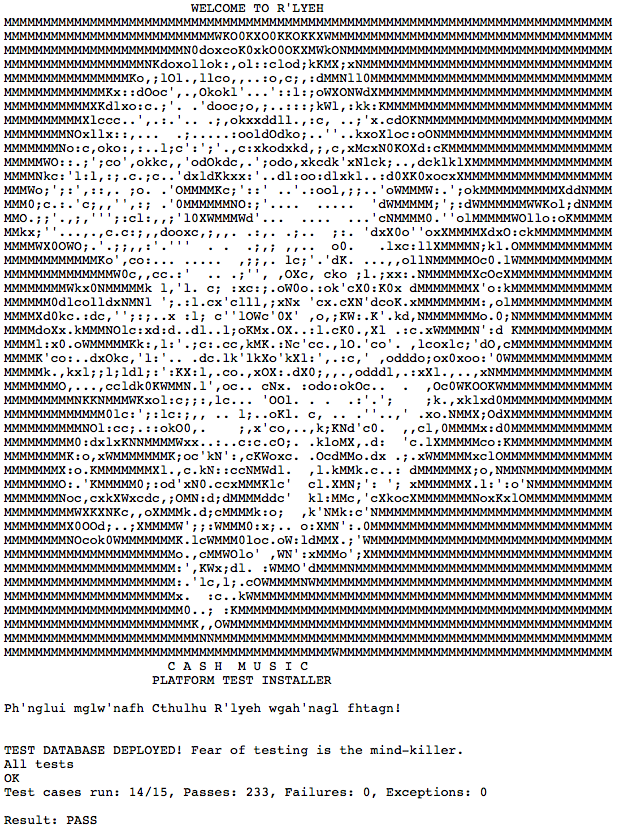
\includegraphics[scale=0.25]{cthulhu_cashmusic}
    \end{center}
}

\frame{
    \frametitle{What does failing test output look like?}
    \begin{center}
        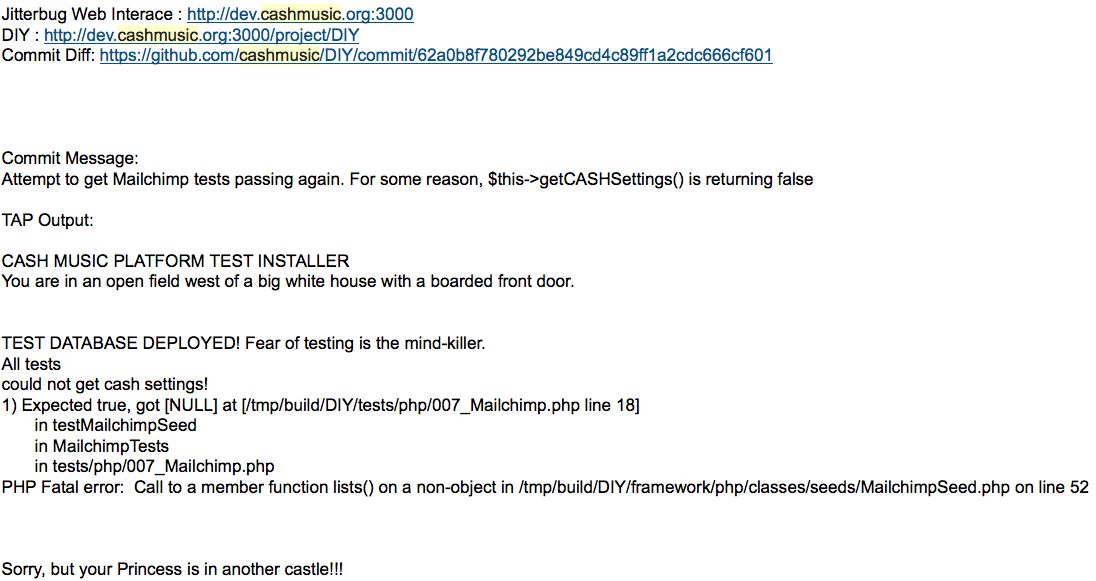
\includegraphics[scale=0.25]{cm_fail}
    \end{center}
}

\frame{
    \frametitle{Future Goals: CASH Music Testing}
    \begin{itemize}
        \item Javascript Unit Tests
        \item Testing the Dev Installer
        \item Javascript Integration Tests
        \item Multi-Browser Integration Testing
    \end{itemize}
}

\frame{
    \frametitle{ Thanks! }
    \begin{itemize}
        \item Jesse + Maggie
        \item Pascal + Diane
        \item WebFWD Fellows + Scouts!
        \item Franck Cuny
    \end{itemize}
}

\frame{
    \frametitle{ Stalk Me }
    \begin{center}
        \begin{itemize}
           \item http://dukeleto.pl
           \item @dukeleto / !leto on twitter/identi.ca
           \item http://linkedin.leto.net
           \item Slides available at http://github.com/leto/presentations
        \end{itemize}
    \end{center}
}
\end{document}
